\section{Qualitätsmaßnahmen}

\begin{tcolorbox}[title=Qualitätsmaßnahmen]
    \textbf{Konstruktive} und \textbf{analytische Maßnahmen} helfen, \textbf{Qualitätsforderungen} einzuhalten:

    \begin{itemize}
            \item  \textbf{Konstruktive Maßnahmen} sollen die Entstehung von Defekten, die Fehler verursachen, verhindern.
            \begin{itemize}
                \item \textbf{Organisatorische Verfahren}: Richtlinien, Checklisten, Standards.
                \item \textbf{technische Verfahren}: technische Qualitätsmaßnahmen wie Methoden, Werkzeuge, Einsatz anderer Programmiersprachen.
            \end{itemize}
            \item \textbf{Analytische Maßnahmen} werden eingesetzt, um entstandene Defekte zu entdecken, damit sie anschließend beseitigt werden können.
            \begin{itemize}
                \item \textbf{analysierende Maßnahmen}: Prüfgegenstand wird systematisch untersucht, ohne ihn in Funktion zu nehmen.\\
                Hierzu werden \textbf{manuelle} und \textbf{werkzeuggestützte Maßnahmen} sowie die \textbf{Verifikation} als analysierende Maßnahmen verwendet:
                \begin{itemize}
                    \item \textbf{manuelle Maßnahmen}: Menschen \textit{lesen} und \textit{analysieren} Prüfgegenstände.
                    \item \textbf{werkzeuggestützte Maßnahmen}: Analysen werden maschinell von Software durchgeführt.
                    \item \textbf{Verifikation}: Nachweis der Richtigkeit von Quellcode durch mathematische Verfahren.
                \end{itemize}
                \item  \textbf{testende Maßnahmen}: Prüfgegenstand wird in Betrieb genommen, das \textbf{beobachtete Verhalten} wird mit dem \textbf{spezifizierten Verhalten} verglichen (\textbf{dynamischer Test})
            \end{itemize}
        \end{itemize}


\end{tcolorbox}


\begin{figure}
    \centering
    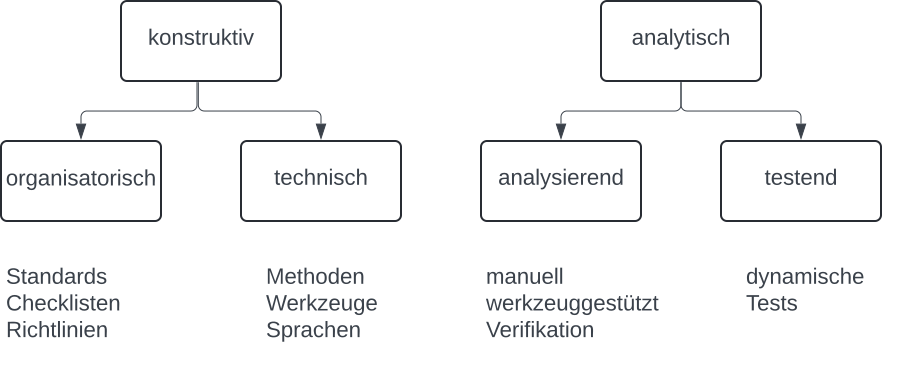
\includegraphics[scale=0.4]{part four/Typen von Qualitätsmaßnahmen/img/systematik qualitätsmaßnahmen}
    \caption{Systematik der Typen von Qualitätsmaßnahmen. (Quelle: in Anlehnung an~\cite[Abb. 2.1, 8]{Wed09c})}
    \label{fig:systematik qualitätsmaßnahmen-cc}
\end{figure}